%% uncomment to list all files in log
%\listfiles

\documentclass[12pt]{report}


\usepackage{fontspec}

%\setmainfont[Scale=MatchLowercase]{Lucida Bright}
%\setmonofont{FreeMono}
%\setmonofont{Source Code Pro}
\setmonofont[Scale=MatchLowercase]{Ubuntu Mono}

\usepackage[headings]{fullpage}

% national use characters 
%\usepackage{inputenc}

% ams mathematical symbols
\usepackage{amsmath,amssymb}

% added to support pandoc highlighting
\usepackage{microtype}

\usepackage{makeidx}

% add index and bibliographies to table of contents
\usepackage[nottoc]{tocbibind}

% postscript courier and times in place of cm fonts
%\usepackage{courier}
%\usepackage{times}

% extended coloring
\usepackage{color}
\usepackage[table,dvipsnames]{xcolor}
\usepackage{colortbl}

% advanced date formating
\usepackage{datetime}

%support pandoc code highlighting
\usepackage{fancyvrb}
\DefineShortVerb[commandchars=\\\{\}]{\|}
\DefineVerbatimEnvironment{Highlighting}{Verbatim}{commandchars=\\\{\}}
% Add ',fontsize=\small' for more characters per line

%tango style colors
% \usepackage{framed}
% \definecolor{shadecolor}{RGB}{255,255,255}
% \newenvironment{Shaded}{\begin{snugshade}}{\end{snugshade}}
% \newcommand{\KeywordTok}[1]{\textcolor[rgb]{0.13,0.29,0.53}{\textbf{{#1}}}}
% \newcommand{\DataTypeTok}[1]{\textcolor[rgb]{0.13,0.29,0.53}{{#1}}}
% \newcommand{\DecValTok}[1]{\textcolor[rgb]{0.00,0.00,0.81}{{#1}}}
% \newcommand{\BaseNTok}[1]{\textcolor[rgb]{0.00,0.00,0.81}{{#1}}}
% \newcommand{\FloatTok}[1]{\textcolor[rgb]{0.00,0.00,0.81}{{#1}}}
% \newcommand{\CharTok}[1]{\textcolor[rgb]{0.31,0.60,0.02}{{#1}}}
% \newcommand{\StringTok}[1]{\textcolor[rgb]{0.31,0.60,0.02}{{#1}}}
% \newcommand{\CommentTok}[1]{\textcolor[rgb]{0.56,0.35,0.01}{\textit{{#1}}}}
% \newcommand{\OtherTok}[1]{\textcolor[rgb]{0.56,0.35,0.01}{{#1}}}
% \newcommand{\AlertTok}[1]{\textcolor[rgb]{0.94,0.16,0.16}{{#1}}}
% \newcommand{\FunctionTok}[1]{\textcolor[rgb]{0.00,0.00,0.00}{{#1}}}
% \newcommand{\RegionMarkerTok}[1]{{#1}}
% \newcommand{\ErrorTok}[1]{\textbf{{#1}}}
% \newcommand{\NormalTok}[1]{{#1}}

%espresso style colors
% \usepackage{framed}
% \definecolor{shadecolor}{RGB}{42,33,28}
% \newenvironment{Shaded}{\begin{snugshade}}{\end{snugshade}}
% \newcommand{\KeywordTok}[1]{\textcolor[rgb]{0.26,0.66,0.93}{\textbf{{#1}}}}
% \newcommand{\DataTypeTok}[1]{\textcolor[rgb]{0.74,0.68,0.62}{\underline{{#1}}}}
% \newcommand{\DecValTok}[1]{\textcolor[rgb]{0.27,0.67,0.26}{{#1}}}
% \newcommand{\BaseNTok}[1]{\textcolor[rgb]{0.27,0.67,0.26}{{#1}}}
% \newcommand{\FloatTok}[1]{\textcolor[rgb]{0.27,0.67,0.26}{{#1}}}
% \newcommand{\CharTok}[1]{\textcolor[rgb]{0.02,0.61,0.04}{{#1}}}
% \newcommand{\StringTok}[1]{\textcolor[rgb]{0.02,0.61,0.04}{{#1}}}
% \newcommand{\CommentTok}[1]{\textcolor[rgb]{0.00,0.40,1.00}{\textit{{#1}}}}
% \newcommand{\OtherTok}[1]{\textcolor[rgb]{0.74,0.68,0.62}{{#1}}}
% \newcommand{\AlertTok}[1]{\textcolor[rgb]{1.00,1.00,0.00}{{#1}}}
% \newcommand{\FunctionTok}[1]{\textcolor[rgb]{1.00,0.58,0.35}{\textbf{{#1}}}}
% \newcommand{\RegionMarkerTok}[1]{\textcolor[rgb]{0.74,0.68,0.62}{{#1}}}
% \newcommand{\ErrorTok}[1]{\textcolor[rgb]{0.74,0.68,0.62}{\textbf{{#1}}}}
% \newcommand{\NormalTok}[1]{\textcolor[rgb]{0.74,0.68,0.62}{{#1}}}

%kete style colors
% \newenvironment{Shaded}{}{}
% \newcommand{\KeywordTok}[1]{\textbf{{#1}}}
% \newcommand{\DataTypeTok}[1]{\textcolor[rgb]{0.50,0.00,0.00}{{#1}}}
% \newcommand{\DecValTok}[1]{\textcolor[rgb]{0.00,0.00,1.00}{{#1}}}
% \newcommand{\BaseNTok}[1]{\textcolor[rgb]{0.00,0.00,1.00}{{#1}}}
% \newcommand{\FloatTok}[1]{\textcolor[rgb]{0.50,0.00,0.50}{{#1}}}
% \newcommand{\CharTok}[1]{\textcolor[rgb]{1.00,0.00,1.00}{{#1}}}
% \newcommand{\StringTok}[1]{\textcolor[rgb]{0.87,0.00,0.00}{{#1}}}
% \newcommand{\CommentTok}[1]{\textcolor[rgb]{0.50,0.50,0.50}{\textit{{#1}}}}
% \newcommand{\OtherTok}[1]{{#1}}
% \newcommand{\AlertTok}[1]{\textcolor[rgb]{0.00,1.00,0.00}{\textbf{{#1}}}}
% \newcommand{\FunctionTok}[1]{\textcolor[rgb]{0.00,0.00,0.50}{{#1}}}
% \newcommand{\RegionMarkerTok}[1]{{#1}}
% \newcommand{\ErrorTok}[1]{\textcolor[rgb]{1.00,0.00,0.00}{\textbf{{#1}}}}
% \newcommand{\NormalTok}[1]{{#1}}
%end pandoc code hacks

% jodliterate colors
\usepackage{color}
\definecolor{shadecolor}{RGB}{248,248,248}
% j control structures 
\definecolor{keywcolor}{rgb}{0.13,0.29,0.53}
% j explicit arguments x y m n u v
\definecolor{datacolor}{rgb}{0.13,0.29,0.53}
% j numbers - all types see j.xml
\definecolor{decvcolor}{rgb}{0.00,0.00,0.81}
\definecolor{basencolor}{rgb}{0.00,0.00,0.81}
\definecolor{floatcolor}{rgb}{0.00,0.00,0.81}
% j local assignments
\definecolor{charcolor}{rgb}{0.31,0.60,0.02}
\definecolor{stringcolor}{rgb}{0.31,0.60,0.02}
\definecolor{commentcolor}{rgb}{0.56,0.35,0.01}
% primitive adverbs and conjunctions
%\definecolor{othercolor}{rgb}{0.56,0.35,0.01}   
\definecolor{othercolor}{RGB}{0,0,255}
% global assignments
\definecolor{alertcolor}{rgb}{0.94,0.16,0.16}
% primitive J verbs and noun names
\definecolor{funccolor}{rgb}{0.00,0.00,0.00}    

\usepackage{framed}
\newenvironment{Shaded}{}{}
\newcommand{\KeywordTok}[1]{\textcolor{keywcolor}{\textbf{{#1}}}}
\newcommand{\DataTypeTok}[1]{\textcolor{datacolor}{{#1}}}
%\newcommand{\DecValTok}[1]{\textcolor{decvcolor}{{#1}}}
\newcommand{\DecValTok}[1]{{#1}} 
\newcommand{\BaseNTok}[1]{\textcolor{basencolor}{{#1}}}
\newcommand{\FloatTok}[1]{\textcolor{floatcolor}{{#1}}}
\newcommand{\CharTok}[1]{\textcolor{charcolor}{\textbf{{#1}}}}
\newcommand{\StringTok}[1]{\textcolor{stringcolor}{{#1}}}
\newcommand{\CommentTok}[1]{\textcolor{commentcolor}{\textit{{#1}}}}
\newcommand{\OtherTok}[1]{\textcolor{othercolor}{{#1}}} 
\newcommand{\AlertTok}[1]{\textcolor{alertcolor}{\textbf{{#1}}}}
%\newcommand{\FunctionTok}[1]{\textcolor{funccolor}{{#1}}}
\newcommand{\FunctionTok}[1]{{#1}}
\newcommand{\RegionMarkerTok}[1]{{#1}}
\newcommand{\ErrorTok}[1]{\textbf{{#1}}}
\newcommand{\NormalTok}[1]{{#1}}

% headers and footers
\usepackage{fancyhdr}
\pagestyle{fancy}

\fancyhead{}
\fancyfoot{}

%\fancyhead[LE,RO]{\slshape \rightmark}
%\fancyhead[LO,RE]{\slshape \leftmark}
\fancyfoot[C]{\thepage}
%\headrulewidth 0.4pt
%\footrulewidth 0 pt

%\addtolength{\headheight}{\baselineskip}

%\lfoot{\emph{Analyze the Data not the Drivel}}
%\rfoot{\emph{\today}}

% subfigure handles figures that contain subfigures
%\usepackage{color,graphicx,subfigure,sidecap}
\usepackage{graphicx,sidecap}
\usepackage{subfigure}
\graphicspath{{./inclusions/}}

% floatflt provides for text wrapping around small figures and tables
\usepackage{floatflt}

% tweak caption formats 
\usepackage{caption} 
\usepackage{sidecap}
%\usepackage{subcaption} % not compatible with subfigure

\usepackage{rotating} % flip tables sideways

% complex footnotes
%\usepackage{bigfoot}

% weird logos \XeLaTeX
\usepackage{metalogo}

% source code listings
\usepackage{listings}

% long tables
% \usepackage{longtable}

\newcommand{\HRule}{\rule{\linewidth}{0.5mm}}

% map LaTeX cross references into PDF cross references
\usepackage[
            %dvips,
            colorlinks,
            linkcolor=blue,
            citecolor=blue,
            urlcolor=blue,   % magenta, cyan default        
            pdfauthor={John D. Baker},
            pdftitle={Analyze the Data not the Drivel},
            pdfsubject={Blog},
            pdfcreator={MikTeX+LaTeXe with hyperref package},
            pdfkeywords={blog,wordpress},
            ]{hyperref}
           
% custom colors
\definecolor{CodeBackGround}{cmyk}{0.0,0.0,0,0.05}    % light gray
\definecolor{CodeComment}{rgb}{0,0.50,0.00}           % dark green {0,0.45,0.08}
\definecolor{TableStripes}{gray}{0.9}                 % odd/even background in tables

\lstdefinelanguage{bat}
{morekeywords={echo,title,pushd,popd,setlocal,endlocal,off,if,not,exist,set,goto,pause},
sensitive=True,
morecomment=[l]{rem}
}

\lstdefinelanguage{jdoc}
{
morekeywords={},
otherkeywords={assert.,break.,continue.,for.,do.,if.,else.,elseif.,return.,select.,end.
,while.,whilst.,throw.,catch.,catchd.,catcht.,try.,case.,fcase.},
sensitive=True,
morecomment=[l]{NB.},
morestring=[b]',
morestring=[d]',
}

% latex size ordering - can never remember it
% \tiny
% \scriptsize
% \footnotesize
% \small
% \normalsize
% \large
% \Large
% \LARGE
% \huge
% \Huge
 
% listings package settings  
\lstset{%
  language=jdoc,                                % j document settings
  basicstyle=\ttfamily\footnotesize,            
  keywordstyle=\bfseries\color{keywcolor}\footnotesize,
  identifierstyle=\color{black},
  commentstyle=\slshape\color{CodeComment},     % colored slanted comments
  stringstyle=\color{red}\ttfamily,
  showstringspaces=false,                       
  %backgroundcolor=\color{CodeBackGround},       
  frame=single,                                
  framesep=1pt,                                 
  framerule=0.8pt,                             
  rulecolor=\color{CodeBackGround},   
  showspaces=false,
  %columns=fullflexible,
  %numbers=left,
  %numberstyle=\footnotesize,
  %numbersep=9pt,
  tabsize=2,
  showtabs=false,
  captionpos=b
  breaklines=true,                              
  breakindent=5pt                              
}

\lstdefinelanguage{JavaScript}{
  keywords={typeof, new, true, false, catch, function, return, null, catch, switch, var, if, in, while, do, else, case, break},
  ndkeywords={class, export, boolean, throw, implements, import, this},
  ndkeywordstyle=\color{darkgray}\bfseries,
  sensitive=false,
  comment=[l]{//},
  morecomment=[s]{/*}{*/},
  morestring=[b]',
  morestring=[b]"
}

% C# settings
\lstdefinestyle{sharpc}{
language=[Sharp]C,
basicstyle=\ttfamily\scriptsize, 
keywordstyle=\bfseries\color{keywcolor}\scriptsize,
framerule=0pt
}

% for source code listing longer than two use smaller font
\lstdefinestyle{smallersource}{
basicstyle=\ttfamily\scriptsize, 
keywordstyle=\bfseries\color{keywcolor}\scriptsize,
framerule=0pt
}

\lstdefinestyle{resetdefaults}{
language=jdoc,
basicstyle=\ttfamily\footnotesize,  
keywordstyle=\bfseries\color{keywcolor}\footnotesize,                                                               
framerule=0.8pt 
}

% APL UTF8 code points listed for lstlisting processing
\makeatletter
\lst@InputCatcodes
\def\lst@DefEC{%
 \lst@CCECUse \lst@ProcessLetter
  ^^80^^81^^82^^83^^84^^85^^86^^87^^88^^89^^8a^^8b^^8c^^8d^^8e^^8f%
  ^^90^^91^^92^^93^^94^^95^^96^^97^^98^^99^^9a^^9b^^9c^^9d^^9e^^9f%
  ^^a0^^a1^^a2^^a3^^a4^^a5^^a6^^a7^^a8^^a9^^aa^^ab^^ac^^ad^^ae^^af%
  ^^b0^^b1^^b2^^b3^^b4^^b5^^b6^^b7^^b8^^b9^^ba^^bb^^bc^^bd^^be^^bf%
  ^^c0^^c1^^c2^^c3^^c4^^c5^^c6^^c7^^c8^^c9^^ca^^cb^^cc^^cd^^ce^^cf%
  ^^d0^^d1^^d2^^d3^^d4^^d5^^d6^^d7^^d8^^d9^^da^^db^^dc^^dd^^de^^df%
  ^^e0^^e1^^e2^^e3^^e4^^e5^^e6^^e7^^e8^^e9^^ea^^eb^^ec^^ed^^ee^^ef%
  ^^f0^^f1^^f2^^f3^^f4^^f5^^f6^^f7^^f8^^f9^^fa^^fb^^fc^^fd^^fe^^ff%
  ^^^^20ac^^^^0153^^^^0152%
  ^^^^20a7^^^^2190^^^^2191^^^^2192^^^^2193^^^^2206^^^^2207^^^^220a%
  ^^^^2218^^^^2228^^^^2229^^^^222a^^^^2235^^^^223c^^^^2260^^^^2261%
  ^^^^2262^^^^2264^^^^2265^^^^2282^^^^2283^^^^2296^^^^22a2^^^^22a3%
  ^^^^22a4^^^^22a5^^^^22c4^^^^2308^^^^230a^^^^2336^^^^2337^^^^2339%
  ^^^^233b^^^^233d^^^^233f^^^^2340^^^^2342^^^^2347^^^^2348^^^^2349%
  ^^^^234b^^^^234e^^^^2350^^^^2352^^^^2355^^^^2357^^^^2359^^^^235d%
  ^^^^235e^^^^235f^^^^2361^^^^2362^^^^2363^^^^2364^^^^2365^^^^2368%
  ^^^^236a^^^^236b^^^^236c^^^^2371^^^^2372^^^^2373^^^^2374^^^^2375%
  ^^^^2377^^^^2378^^^^237a^^^^2395^^^^25af^^^^25ca^^^^25cb%  
  ^^00}
\lst@RestoreCatcodes
\makeatother

% custom lengths used within minipages
\newcommand{\minindent}{17pt}


\makeindex

\begin{document}

\subsection*{\href{https://bakerjd99.wordpress.com/2014/10/30/photospheres-away-2/}{Photospheres Away!}}
\addcontentsline{toc}{subsection}{Photospheres Away!}


\noindent\emph{Posted: 30 Oct 2014 16:53:30}
\vspace{6pt}

Photographers are notorious gearheads. Everybody has a favorite lens,
camera, or tripod, and no matter how much gear we have, more is always
better! Hey, somebody has to stimulate the moribund Obama economy. Gear
lust is not entirely irrational. Good cameras really do take
``technically'' better pictures than mediocre or poor cameras, but here's
the infuriating thing. Technical merit does not make the image!

Image quality depends on many things and changes over time. If you doubt
this, imagine you have an old locket that frames~a
\href{https://en.wikipedia.org/wiki/Daguerreotype}{Daguerreotype} of
your great-great-grandmother. I'd bet that every single portrait on your
shiny new iPhone is ``technically'' superior to that old Daguerreotype
, but I'd also bet you'd chuck your iPhone before giving up that old
Daguerreotype. An image's quality goes far beyond
\href{http://photographylife.com/how-to-read-mtf-charts}{MTF curves} and
pixel counts. Photography and geometry are both bereft of royal roads.

In the early days of photography, gear was a serious constraint. Getting
a good picture was a technical and artistic struggle. Imagine shooting a
panorama using large glass plates covered with a home-brewed
\href{http://www.alternativephotography.com/wp/processes/gelatin-silver/silver-gelatin-dry-plate-process}{ASA
0.5}, (you read that right, ASA 0.5), blue light-sensitive emulsion.
Despite such limitations, early photographers managed to create some
great images. Imagination and gumption have always been the most
important photographic tools, with good lenses as a distant third. Well,
the 150-year reign of the lens has ended, \emph{software has displaced
the lens as the primary modern photographic tool} and
\href{https://itunes.apple.com/us/app/photo-sphere-camera/id904418768}{Google's
Photosphere} cell phone application neatly demonstrates this
technological shift.

\captionsetup[figure]{labelformat=empty}
\begin{figure}[htbp]
\centering
\href{http://conceptcontrol.smugmug.com/Themes/Manipulations/Panoramas-1}{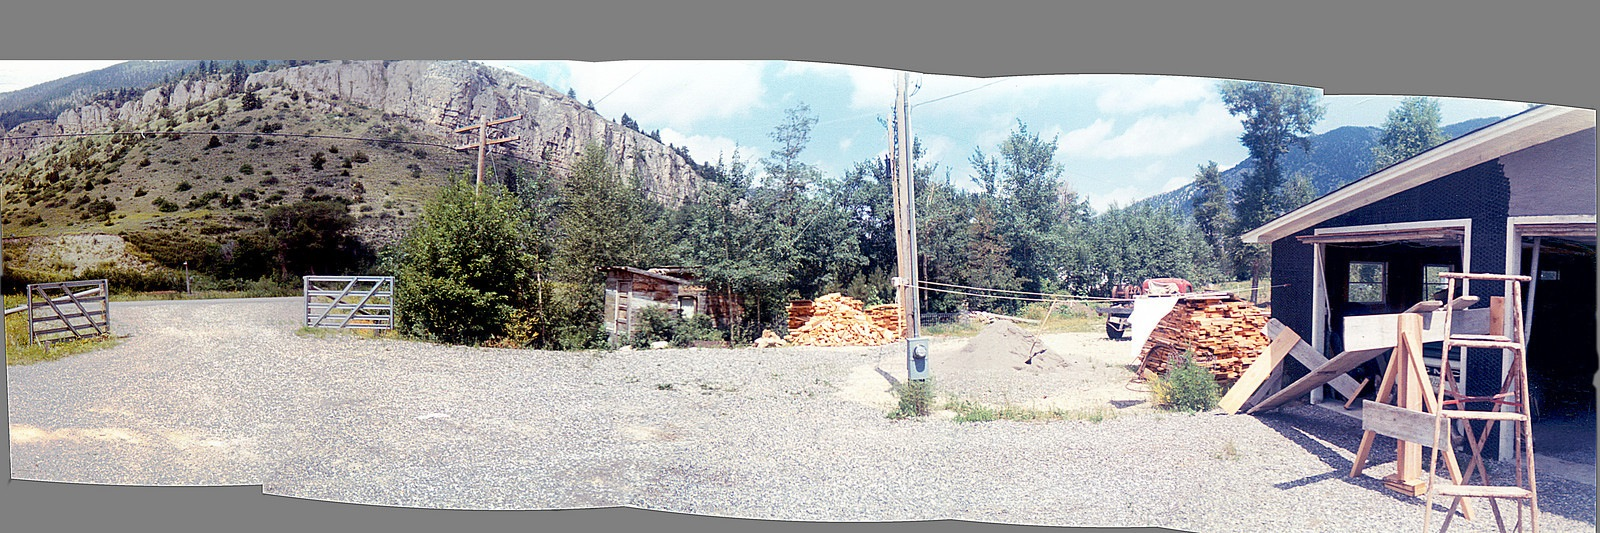
\includegraphics[width=0.75\textwidth]{gert-driveway.jpg}}
\caption[I shot this panorama in the 1960s]{I shot this panorama in the 1960s. I rotated in my grandfather's
driveway, shooting an entire roll of film with my Instamatic camera. Many
years later, I scanned the prints and used panorama software to stitch
the images together. Click on the image for more
panoramas.}
\label{fig:4832X0}
\end{figure}


A
\href{https://www.google.com/maps/about/contribute/photosphere/}{photosphere}
is a panorama on steroids. It's a complete 360-degree look-around image.
The Google Photosphere app derives from Google Maps street view. Street
views are shot with special multi-lens cameras that look everywhere at
once, but some bright spark in Google realized that you could get roughly
the same result from a single lens if the photographer was willing to
endure a vertigo-inducing dance. Shooting a photosphere takes at least
three twirling 360-degree passes. You have to shoot the ground, horizon
, and sky. It takes about twenty frames to build a photosphere.

There is nothing new about multi-frame panoramas. Photographers started
shooting multi-frame panoramas
\href{https://content.lib.washington.edu/panoramweb/history.html}{shortly
after the camera's invention}. I shot them when I was a teenager. Panorama
software isn't new either; it's been around for decades. Two ``new''
developments make photospheres possible: photosphere viewers and cameras
(cell phones), that are more software than camera.



%{[}caption id=``attachment\_4842'' align=``aligncenter''  width=``584''{]}
%\href{http://bakerjd99.wordpress.com/2014/10/30/photospheres-away-2/gert-driveway-2/}{\includegraphics{gert-driveway1.jpg}}
%I shot this panorama in the 1960s. I rotated in my grandfather's
%driveway shooting an entire roll of film with my Instamatic camera. Many
%years later I scanned the prints and used panorama software to stitch
%the images together. Click on the image for more
%panoramas.
%{[}/caption{]}


The sphere cannot be mapped onto the plane without distortion. This
mathematical fact limits how wide-angle your wide-angle shots can be
before they are unnaturally distorted. A flattened 360-degree view of
common rectilinear subjects looks wonderfully, or horribly, weird:
straight lines become curves, and areas lose proportionality. Many
natural vistas can tolerate such torments, but average street views
cannot. Photosphere viewers fix this problem by simulating how we look
around. Every time you browse a Google Street View you are running a
photosphere viewer.


\begin{figure}[htbp]
\centering
\href{https://www.google.com/maps/views/view/109459250977988268850/gphoto/6071702564097759170}{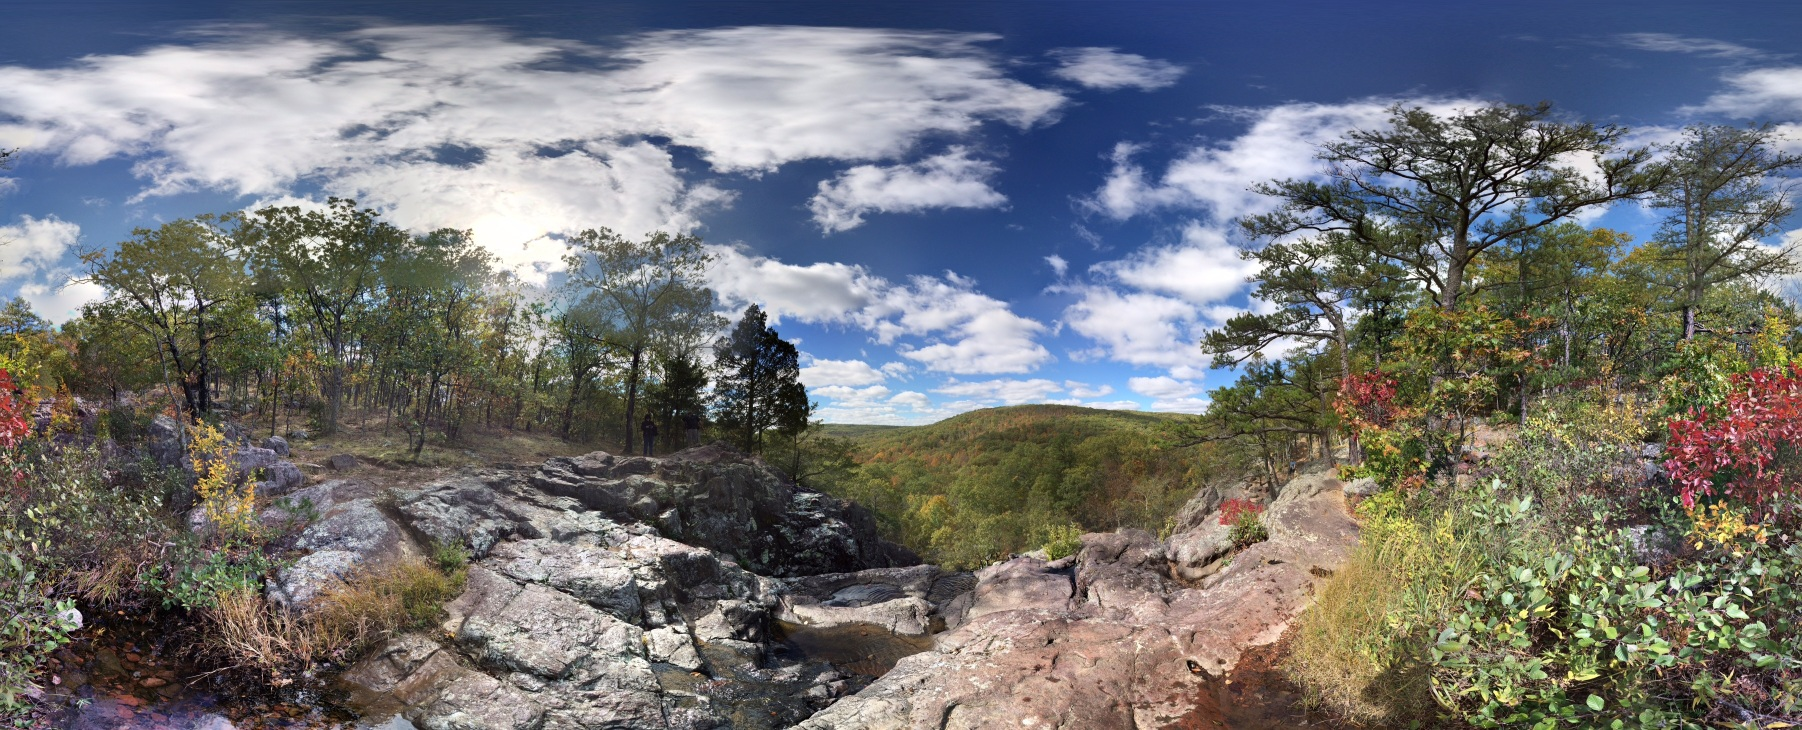
\includegraphics[width=0.75\textwidth]{arcadia-photosphere.jpg}}
\caption[Photosphere of a waterfall in Taum Sauk park Arcadia Missouri]{A photosphere at the top of a waterfall in Taum Sauk state park near Arcadia Missouri.
Click for a 360 photosphere viewer.}
\label{fig:4832X0}
\end{figure}


%{[}googlemaps  https://maps.google.com/maps?layer=c\&panoid=lcPAeYAkFhMAAAQYkFYXSw\&ie=UTF8\&source=embed\&output=svembed\&cbp=13\%2C354.06759999999997\%2C\%2C0\%2C0\&w=560\&h=315{]}


%\href{https://www.google.com/maps/views/}{Views}:
%\href{https://www.google.com/maps/views/view/109459250977988268850/gphoto/6071702564097759170}{Palmer
%Creek, Arcadia, MO} by
%\href{https://www.google.com/maps/views/profile/109459250977988268850}{John
%Baker}

Shooting panoramas and photospheres is like any other type of
photography. It takes lots of practice! It was hard to ``practice''
shooting such images before cell phones could run stitching and viewing
software because you couldn't see what you had until you took your
twenty frames back to the ``lab'' and tediously put them together. Ten
years ago, panorama software required a lot of manual intervention. I
spent hours putting three or four frames together. I didn't put a twenty
frame together until I snapped my first iPhone Photosphere.

The iPhone lens is a pretty crappy short focal-length lens. Any decent
camera lens easily outclasses it yet I cannot shoot photospheres with my
expensive Nikon's while my cruddy little cell phone can.~ What's the
difference?~ Software!

\begin{figure}[htbp]
\centering
\href{https://www.google.com/maps/views/view/109459250977988268850/gphoto/6074254717471563618}{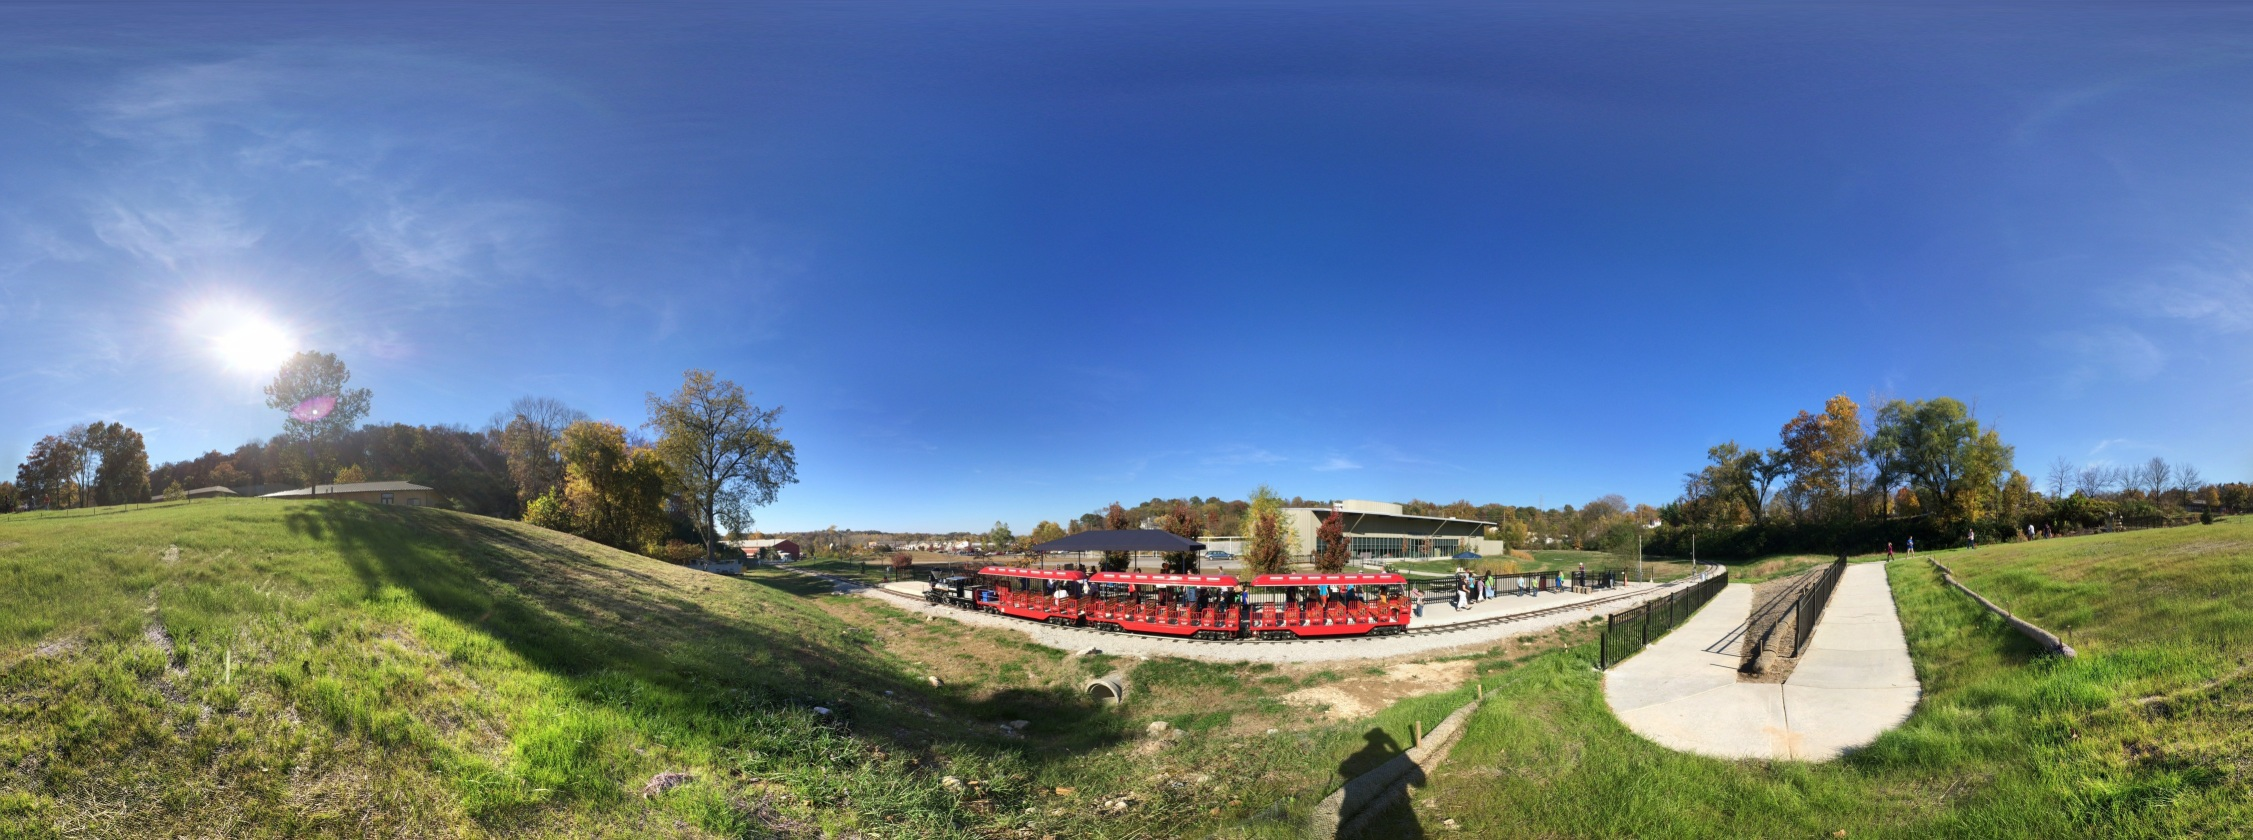
\includegraphics[width=0.75\textwidth]{museum-photosphere.jpg}}
\caption[Photosphere of the Museum of Transportation in Saint Louis]{A photosphere on the grounds of the Museum of Transportation in Saint Louis Missouri.
Click for a 360 photosphere viewer.}
\label{fig:4832X0}
\end{figure}


%{[}googlemaps  https://maps.google.com/maps?layer=c\&panoid=7eGAlcZ-94MAAAQYgcRcww\&ie=UTF8\&source=embed\&output=svembed\&cbp=13\%2C83.01108972943024\%2C\%2C0\%2C11.599426335166598\&w=560\&h=315{]}


%\href{https://www.google.com/maps/views/}{Views}:
%\href{https://www.google.com/maps/views/view/109459250977988268850/gphoto/6071703165223689154}{Pilot
%Knob, MO} by
%\href{https://www.google.com/maps/views/profile/109459250977988268850}{John
%Baker}

iPhone Google photospheres are fun, but they're flaw-ridden. You can
easily see stitching errors, blending artifacts, ghost people, and other
blemishes. Now that we can shoot photospheres, the race is on to shoot
quality photospheres! Software will dominate, but hardware has to catch
up to make this happen. Before long, you will be able to buy a special
multi-lens photosphere ball camera that you can literally throw into the
air. This ought to fix the viewpoint problem for people with good
pitching arms, and the rest of us can drop the little sucker from a
drone. Photospheres away!

\begin{SCfigure}[10]
\centering
\href{http://www.dpreview.com/articles/9435374316/panono-announces-pricing-and-availability-for-rolling-ball-camera}{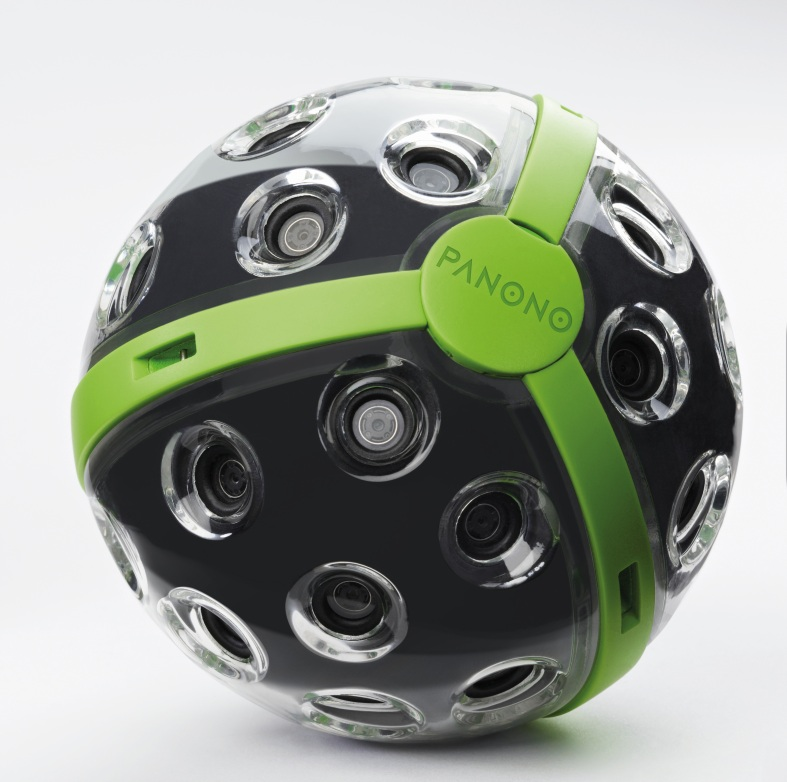
\includegraphics[width=0.23\textwidth]{panono-ball-camera.jpg}}
\caption[The Panono ball is a multi-lens camera that shoots 
photospheres]{The Panono ball camera is a small multi-lens camera that shoots 360
photospheres by simultaneously capturing images from all its lenses and
stitching the result together. It is designed to be thrown into the air.
Photosphere baseball is going to be huge!}
\label{fig:4832X1}
\end{SCfigure}


%{[}caption id=``attachment\_4848'' align=``aligncenter''  width=``200''{]}
%\href{http://www.dpreview.com/articles/9435374316/panono-announces-pricing-and-availability-for-rolling-ball-camera}{\includegraphics{panono-ball-camera1.jpg}}
%The Panono ball camera is a small multi-lens camera that shoots 360
%photospheres by simultaneously capturing images from all its lens and
%stitching the result together. It is designed to be thrown into the air.
%Photosphere baseball is going to be huge!
%{[}/caption{]}


%\captionsetup[floatingfigure]{labelformat=empty}
%\begin{figure}[htbp]
%\begin{floatingfigure}[l]{0.25\textwidth}
%\centering
%\includegraphics[width=0.23\textwidth]{gert-driveway1.jpg}
%\caption{~~~IMCAPTION~~~}
%\label{fig:4832X0}
%\end{floatingfigure}
%\end{figure}

%\captionsetup[floatingfigure]{labelformat=empty}
%\begin{figure}[htbp]
%\begin{floatingfigure}[l]{0.25\textwidth}
%\centering
%\includegraphics[width=0.23\textwidth]{panono-ball-camera1.jpg}
%\caption{~~~IMCAPTION~~~}
%\label{fig:4832X1}
%\end{floatingfigure}
%\end{figure}



%\end{document}